The low Reynolds number is called the creeping, or over-damped
regime. Let us generalize slightly the momentum equation
Eq \ref{eq:NS_usual} to a general volumetric external force $\bff$:
\[
  \rho \frac{d\bfu }{dt} =
  - \nabla p 
  + \mu \nabla^2 \bfu
  + \bff .
\]

We may again cast the equation into reduced form, to get
\[
\rho^* \frac{d\bfu^* }{dt^* } =
-  \nabla^* p^*
+  \frac1{\mathrm{Re}} \nabla^{*2} \bfu^* .
+  \bff^* ,
\]
where $\bff^*= L/(\rho_0 u_0^2) \bff$. 

As $\mathbf{Re}$ is very small, the equation will tend to
\[
0 = - \mathrm{Re} \nabla^* p^* + \nabla^2 \bfu^* + \mathrm{Re} \bff^*
.
\]
All time derivatives are gone from the equation! The only time
variation that is sometimes considered is the case in which $\bff^*$
is a explicit function of time. In this case, the velocity field
adapts instantaneously following the changes in external force. Coming
from previous chapters, devoted to cases where intertial effects are
not negligible, this may come as a surprise --- nevertheless, this is
the correct description of a regime which is important in fields such
as microfluidics and the biological physics of small systems (from
small insects down to large molecules).  Mathematically, the resulting
equation is now linear in the velocity, which makes its treatment
simpler.

An objection could be raised regarding why the pressure gradient and
the external force terms are kept in the equation, despite being
multiplied by the Reynolds number. The answer is that they are not
in fact negligible, as an alternative scaling is employed. This is
discussed in the next section.



\subsection{Kolmogorov flow}

In order to get an idea of the features of the flow (typical speed,
time scale, Reynolds number), we may gain some insight from the
solution from Kolmogorov flow.

This is an exact solution of the momentum equations when there is a
periodic applied force in the $x$ direction that depends on $y$ only
\[
\bff = f_0 \cos\left( \frac{2\pi y}{L} \right) \bfe_x .
\]

In this case, the typical length-scale $L_0$ and velocity $u_0$ are
set by the force. The former is clearly $L_0=L$, but the velocity is
actually part of the solution. It is therefore more convenient to
introduce an alternative way to cast the momentum equation in
non-dimensional form. First, dividing by $f_0$ and going to
dimensionless spacial coordinates:
\begin{equation}
\label{eq:Navier-Stokes_nondim1}
\frac{\rho}{f_0}
\frac{d \bfu}{d t} =
\frac\mu{f_0 L^2} (\nabla^*)^2 \bfu
-\frac 1{f_0 L} \nabla^* p + \bff^*(\bfr^*) .
\end{equation}
The viscous term sets the velocity scale:
\begin{equation}
  \label{eq:reduced_u0}
  u_0 = ( f_0 L^2 ) / \mu .
\end{equation}

On the left hand side of \ref{eq:Navier-Stokes_nondim1}, the total
derivative limits the setting of the time scale: $t_0=L/u_0$. This
means the equation may be written as
\[
\frac{\rho L^3 f_0}{\mu^2}
\frac{d \bfu^*}{d t^*} =
(\nabla^*)^2 \bfu^*
-\nabla^* p^* + \bff^*(\bfr^*) ,
\]
or
\begin{equation}
\label{eq:Navier-Stokes_nondim2}
\mathrm{Re}
\frac{d \bfu^*}{d t^*} =
(\nabla^*)^2 \bfu^*
-\nabla^* p^* + \bff^*(\bfr^*) ,
\end{equation}
where we again find the Reynolds number, given as
\[
  \mathbf{Re}=\frac{\rho L^3 f_0 }{\mu^2}.
\]
This definition looks rather different from the standard one,
$ \mathbf{Re}=\rho L u_0 / \mu$, but upon insertion of
the typical velocity both are seen to coincide.

Notice that the reduced response time is given by the Reynolds number.
This is a sort of ``double-reduced'' time, given by
$t^{**}= t^* / \mathbf{Re}$. A high Reynolds number therefore means a
long reduced time to respond, while a low Reynolds one the response is
very rapid, and the equilibrium solution is reached very fast. Also,
the pressure is reduced as $p^*= p / ( f_0 L ) $.

Let us apply this scaling to the Kolmogorov flow. Assuming that the
resulting velocity, as the driving force, only has an $x$ component
varying on $y$ (as for planar Couette and Poiseuille flows),
\begin{equation}
\label{eq:Kolmo_orig}
  \rho \frac{\partial u_x}{\partial t} =
  \mu \frac{\partial u_x}{\partial y^2} - \nabla p +   f_0 \cos(2\pi y/L)  .
\end{equation}

As in previous flow patterns, we may set the pressure to some constant
value. Therefore, in reduced units (dropping the askterisks for
clarity),
\[
  \mathrm{Re} \frac{\partial u_x}{\partial t} =
  \frac{\partial  u_x}{\partial y^2} u + \cos(2\pi y) .
\]

The solution is easily found:
\[
  u_x = \frac{1}{(2\pi)^2} \left( 1-e^{ - (2\pi)^2 t/Re } \right)
  \cos(2\pi y) .
\]

Putting the scales back in, we find
\[
  u = \frac{ f_0 L^2 }{(2\pi)^2 \mu} \left( 1-e^{- (2\pi)^2 \mu t /
      (\rho L^2) } \right) \cos(2\pi y/L) ,
\]
which indeed can be checked to be the solution to the original
Equation \ref{eq:Kolmo_orig}.


\section{General solution}

In Equation \ref{eq:Navier-Stokes_nondim2}, we may disregard
completely the left hand side if the Reynolds number is very low. This
leads to Stokes' equation \index{Stokes' equation}:
%, which in dimensionless units is:
\begin{equation}
  \label{eq:Stokes}
  \mu \nabla^2 \bfu -\nabla p = - \bff(\bfr) .
\end{equation}
As mentioned, this is a \emph{linear} equation for the velocity.  We
may get a general solution to the equation that gives us the velocity
field for any external field, by using Fourier techniques.

In Fourier space all the fields are given as \index{Fourier transform}
\begin{align}
  \label{eq:F_r_to_q}
  \phi_\bfq &=                    \int d\bfr \, \phi(\bfr) e^{-i\bfq\cdot\bfr}  \\
  \label{eq:F_q_to_r}
  \phi(\bfr) &= \frac 1{(2\pi)^d}  \int d\bfq \, \phi_\bfq e^{ i\bfq\cdot\bfr} .
\end{align}
We follow the convention that is usual in physics, in which Fourier
components are indicated by an index --- also, no tilde (``wiggly'')
hat is used for them for simplicity. Thus, $ \phi_\bfq $ instead of
$ \tilde{\phi}(\bfq) $.

Stokes' equation for Cartesian coordinate $i$ reads
\cite{bray2002theory}
\[
-\mu q^2 \bfu_{\bfq,i} - i \bfq_i p_\bfq = - \bff_{\bfq,i} ,
\]
or
\begin{equation}
\label{eq:u_Fourier0}
\bfu_{\bfq,i} = \frac 1{\mu q^2}
\left[
  - i \bfq_i p_\bfq + \bff_{\bfq,i} 
\right] .
\end{equation}

Now, the pressure is fixed by incompressibility. The condition
$\nabla\cdot\bfu=0$, reads in Fourier space
\[
  \sum_i\bfq_i\cdot\bfu_{\bfq,i} .
\]
Multiplying Equation \ref{eq:u_Fourier0} by $\bfq_i$ and adding up the
$d$ equations:
\[
\sum_i \bfq_i \bfu_{\bfq,i} = \frac 1{\mu q^2}
\left[
  - i q^2 p_\bfq + q_i\bff_{\bfq,i} 
\right] =0 .
\]

Therefore,
\[
  - q^2 p_\bfq = i q_i\bff_{\bfq,i}   .
\]
This looks like the Fourier version of a Poisson pressure equation:
\[
  \nabla^2 p = \nabla\cdot \bff .
\]
This is no coincidence, since in \ref{eq:Stokes} we may use the
identity
\(\nabla^2 \bfu = \nabla(\nabla\cdot\bfu -
\nabla\times\nabla\times\bfu \). The first term must be zero for an
incompressible fluid, and applying $\nabla\cdot$ we may get rid of the
first one too (since a rotational field is divergence free). The
Poisson equation results. It is interesting that much the same
equation is found in computational methods that enforce
incompressibility by projection.

The pressure is then
\begin{equation}
\label{eq:p_Fourier0}
p_\bfq = -i \frac{\sum_i q_i\bff_{\bfq,i} }{q^2} .
\end{equation}

With this result we may write Equation \ref{eq:u_Fourier0} as
\begin{equation}
\label{eq:u_sol_Fourier}
\bfu_{\bfq,i} = \frac 1{\mu q^2}
\sum_j
\left[ \delta_{ij} - \frac{ \bfq_i  \bfq_j}{q^2} \right]
\bff_{\bfq,j} =: \sum_j T_{ij} \bff_{\bfq,j},
\end{equation}
%
where the last equation the Oseen tensor is defined:
\[
T_{\bfq,ij} := \frac 1{\eta q^2} \left[
  \delta_{ij} - \frac{ \bfq_i  \bfq_j}{q^2} 
\right].
\]

In 3D, Equation \ref{eq:p_Fourier0} may be inverted back to real space
to yield \cite{pozrikidis2011introduction}.
\[
p(\bfr) = \frac{\bff\cdot\bfr}{4\pi r^3} .
\]

Oseen's tensor can also be inverted:
\[
T_{ij}(\bfr) :=  \frac 1{8\pi \eta r} 
\left(
  \delta_{ij} + \frac{ \bfr_i  \bfr_j}{r^2}
\right)
\]
But notice Equation \ref{eq:u_sol_Fourier} is a convolution in
real space:
\begin{equation}
\label{eq:u_sol_real}
\bfu_i(\bfr) =  \sum_j \int \,d\bfr' T_{ij}(\bfr'-\bfr) \bff_j(\bfr') .
\end{equation}

In 2D, on the other hand, the Fourier expressions cannot be
inverted. This is the famous ``Stokes paradox''\index{Stokes
  paradox''}: there are no solutions to his equation for steady
translational motion in 2D (it also applies to 2D problems in 3D, such
as the motion of an infinite cylinder).


\subsection{Monolayers and membranes}

In their influential 1975 article Saffman and Delbr{\"u}ck
\cite{saffman1975brownian} discussed several ways out of this paradox,
and found out the most satisfactory way was to take into account the
viscosity of the surrounding liquid, $ \mu_\mathbf{f}$.

In \cite{lubensky1996hydrodynamics}, Lubensky and Goldstein proposed a
modification of the original equation for 2D liquids. This are indeed
feasible in a lab, as Langmuir monolayers \index{Langmuir monolayer},
in which a one molecule thick layer of lipids forms between water and
air. Also, in membranes, where a 2D bilayer lipid is surrounded on
both sides by water (these are more involved to study, and may be
prone to curve). The equation of motion, in the creeping regime is
\begin{equation}
  \label{eq:Stokes_2D}
  \mu \nabla^2 \bfu - \nabla p = -\bff(\bfr) -\bff'(\bfr) ,
\end{equation}
%
where all variables are two-dimensional: $\mu$ is the 2D shear
viscosity, $p$ the 2D pressure, and $\bff$ a force per area. All
variables have their physical dimensions changed from the 3D case (and
the rest of this book), but for the position $\bfr$ and the velocity
$\bfu$ --- both are in-plane, but their units do not change: length
and length per time.

Notice that the fluid is taken to be Newtonian, which may not be such
a good approximation for molecules as complex as lipids.  In addition,
the 2D flow is incompressible:
\[
  \nabla\cdot \bfu = 0
\]

The solvent produces an additional term $\bff'(\bfr) $, to be added to
any external force that causes the flow (which may be an external
forcing due to the motion of an immersed body, or perhaps due to a
concentration gradient \cite{duque2018}. Of course, this surrounding
flow is caused by the 2D fluid, so this will be a sort of
self-interaction effect, as we will see.

The solvent itself satisfies another momentum equation. It the solvent
is taken to be also in the creeping regime:
\[
  \mu' \nabla'^2 \bfu' -\nabla' p' = 0 .
\]
In this section, primes refer to volume properties of the solvent
(also for $\nabla'$, which is our usual, 3D, del operator). In this
equation $\mu'$ is the ordinary solvent shear viscosity, often simply
water. It is also taken to be Newtonian, an approximation whose
validity depends on the nature of the solvent. This flow is also
incompressible:
\[
  \nabla'\cdot \bfu' = 0 .
\]

The reader may wonder how the 2D fluid affects the 3D one which is
underneath (this is the case of monolayers, while in membranes there
are two such regions, above and below.) The answer is, through the
boundary condition at the surface:
\[
  \bfu'(z=0) = \bfu .
\]
In addition to this condition, another one must be set. Usually,
disturbances die out quite fast (as we will see below), so the
deep-water limit is a good approximation:
\[
  \bfu'(z \to -\infty ) = 0 .
\]
A more general condition $\bfu'(z = -H ) = 0$ is also easy, but
somewhat obscures the discussion.

Let us consider the 2D Fourier transform of our in-plane velocity
field, $\bfu_\bfq$. The wave-vector $\bfq$ is also a 2D vector. Let us
consider this ansatz for the solvent velocity field:
\[
  \bfu' =  \frac 1{(2\pi)^2}  \int d\bfq \, \bfu_\bfq e^{ i\bfq\cdot\bfr} e^{q z} .
\]
Notice that this is a half-Fourier inverse transform, only in $q_x$
and $q_y$, but not on $q_z$. What we have here is a dilution of each
of the 2D Fourier components $\bfu_\bfq$ as we go deeper into the
solvent, each decaying as $e^{q z} $ (remember, $z$ is
negative!). This means the sharper features will wash out first, and
the longest-wavelength features will be the ones that will extend
deeper.

Notice that this velocity field is laminar: it is always parallel to
the 2D layer (i.e. it has no $z$ component). It automatically
satisfies incompressibility. It is also harmonic: $\nabla^2 \bfu' = 0$
(for this, it is imperative that the decay is precisely
$e^{qz}$. These two facts imply that the pressure field is not needed,
and we may take it to be constant.

Lastly, the force this velocity field will exert on the planar
interface can only be a wall shear stress. Recalling our expressions
for the shear stress on walls, e.g. Eq.  \ref{eq:wall_shear_stress},
the force per unit surface on the 2D fluid will be
\begin{equation*}
  f_x = - \tau_{zx} \qquad
  f_y = - \tau_{zy} \qquad
  f_z = - \tau_{zz} ,
\end{equation*}
since we would be considering only forces on the top wall of the cube
of Fig. \ref{fig:cube_for_stresses}. The minus sign arises because
these forces are the reaction to the forces exerted by the wall upon
the particles closeby. (If this is confusing, recall that in
Poiseuille flow the force upon the walls of Eq \ref{eq:Couette_force}
of course goes \emph{against} the flow.)

Since our fluid is Newtonian, Eqs. \ref{eq:tau_diagonal} and
\ref{eq:tau_off_diagonal} yield
\begin{equation*}
  \tau_{zz} = -p'  \qquad
  \tau_{zx} = \mu' \frac{\partial u'_x}{\partial z}  \qquad
  \tau_{zy} = \mu' \frac{\partial u'_y}{\partial z}  \qquad
\end{equation*}
where many terms have vanished because $\bfu'$ does not have a $z$
component. The second viscosity of Eq. \ref{eq:tau_diagonal} does not
appear since the flow is incompressible. The first equation represents
a push from the constant pressure underneath (recall that minus sign
again), but in an experimental situation this is balanced by either
some external pressure in the case of monolayers (most simply,
atmospheric pressure), or by an equal pressure on the other side for
the case of membranes.

We may combine the two latter expressions to write down a vectorial
equation for the force per unit area on the surface due to the
solvent:
\[
  \bff' = - \mu' \left. \frac{\partial \bfu'}{\partial z} \right|_{z=0} .
\]


With our previous ansatz,
\[
  \bff' = - \frac 1{(2\pi)^2} \mu' \int d\bfq \, q \bfu_\bfq e^{
    i\bfq\cdot\bfr} .
\]

This is a very interesting result. It is clear that the 2D Fourier
transform of the solvent force is
\[
  \bff'_\bfq =  \mu' q \bfu_\bfq .
\]

Therefore, if we cast our original 2D momentum equation
\ref{eq:Stokes_2D} into Fourier space:
\[
-  \mu q^2 \bfu_\bfq - i \bfq p_\bfq = -\bff_\bfq -\bff'_\bfq ,
\]
we have
\[
-  ( \mu q^2 +  \mu' q ) \bfu_\bfq - i \bfq p_\bfq = -\bff_\bfq .
\]

We may now repeat the steps by which we obtained
\ref{eq:u_sol_Fourier}, with the result
\begin{equation*}
\bfu_i(\bfq) =  \sum_j T_{ij} \bff_j(\bfq),
\end{equation*}
%
but now the Oseen tensor is re-defined:
\[
T_{ij}(\bfq) := \frac 1{\mu q^2 +  \mu' q  } \left[
  \delta_{ij} - \frac{ \bfq_i  \bfq_j}{q^2} 
\right].
\]

The denominator is usually written as
\[
  \mu q^2 +  \mu' q =:
  \mu (q^2 +  q \xi ) ,
\]
where $\xi:= \mu'/\mu$ is the Saffman and Delbr{\"u}ck length
\index{Saffman and Delbr{\"u}ck length }. (Remember the two
viscosities have different dimensions, so their ratio is indeed a
length). This length separates two regimes.  One of them is the
high-$q$, short wave-length regime, when $q \gg 1/\xi$. In this case
the effect of the solvent is negligible, as we recover our previous 2D
result. The other is the low-$q$, high wave-length regime, when
$q \ll 1/\xi$. In this case the $q\xi$ term dominates, and the tensor
switches over to a $1/q$ increase which makes it Fourier
invertible. Stokes' paradox is therefore removed! Sadly, the resulting
expressions cannot be annalitically expressed in general (they can in
those two limits.)

For membranes the discussion is exactly the same, with two mirroring
fluid zones above and below the membrane, both of them affecting the
membrane. The only difference is therefore that in this case
\[
T_{ij}(\bfq) = \frac 1{\mu q^2 +  2 \mu' q  } \left[
  \delta_{ij} - \frac{ \bfq_i  \bfq_j}{q^2} 
\right],
\]
and the Saffman and Delbr{\"u}ck length $\xi = 2 \mu'/\mu$.




In Figure \ref{fig:SD} we plot the function $1/(q^2+q)$ in log-log
scale.  At high $q$ (short distances), the denominator approaches
\( \eta_\mathrm{m} q^2 \),
which is the prediction from the standard theory as just described. At
low $q$ (long distances), on the other hand, the denominator
approaches \( 2 \eta_\mathrm{f} q \),
which will cause a convergent real-space Oseen tensor with magnitude
given by the viscosity of the surrounding liquid.

At this stage, I do not know how to implement this correction in real
space, and until I get results I am not convinced it is really that
important.

\begin{figure}
  \centering
  \begin{minipage}{0.45\textwidth}
      \includegraphics[width=\textwidth]{figures/SD}
  \end{minipage}
  \caption{Plot of $1/(q^2+q)$ function
    \label{fig:SD}}
\end{figure}



\section{Creeping flow past a sphere}

Unfortunately, the creeping flow past a cylinder cannot be solved, due
to Stokes paradox. This may have been anticipated by dimensional
analysis. Indeed, the drag force on a sphere of radius $R$ is expected
to be given by
\[
  D \sim \mu u_0 R ,
\]
which has the right combination of units to yield a net force. It also
makes sense, being proportional to the viscosity, velocity, and
radius. (One may have expected $R^2$, the projected area, but this
does not work dimensionally.) It is indeed correct, a fact that will
be proved in this section, together with the missing numerical
prefactor.

If we write something similar for the drag force on a cylinder, the
answer should come as a force per length in the perpendicular
direction (as e.g. the lift for our cylinder with circulation of
\ref{sec:}). I.e.
\[
  \frac{D}{R} \sim \mu u_0 .
\]
But this makes no sense, since all dependence on $R$ is lost --- and
there is not clear candidate to provide another length parameter.

To solve this problem, we begin with the Stokes equation with no
forces:
\begin{equation}
  \label{eq:Stokes}
  \mu \nabla^2 \bfu -\nabla p = 0 .
\end{equation}

We may intruduce the vorticity $\vort=\nabla\times\bfu$, and recall
the expression for the curl of the curl used previously,
Eq. \ref{eq:curl_of_curl},
%
\begin{equation*}
  \nabla \times \vort =
  \nabla (\nabla \cdot \bfu )-\nabla^{2} \bfu .
\end{equation*}

The first term is null due to incompressibility. Hence,
\[
\mu \nabla \times \vort = - \nabla p.
\]
If we take the divergence of this expression we find that the pressure
is harmonic:
\[
  \nabla^2 p = 0
\]

If, on the other hand, we take the curl, we find
\[
  \nabla \times \left(\nabla \times \vort \right)= 0
\]
This is again, the curl of a curl, so Eq. \ref{eq:curl_of_curl} may be
again used:
\begin{equation*}
  \nabla \times \left(\nabla \times \vort \right)=
  \nabla (\nabla \cdot \vort )-\nabla^{2}\vort .
\end{equation*}
But the vorticity is always divergence-free, it being the curl of
another field. Therefore vorticity is also harmonic!:
\[
  \nabla^2 \vort = 0 .
\]

Our method of solution will make use of the stream
function. Introducing our vector potential of
Eq. \ref{eq:vector_potential}
\[
  \vort = \nabla \times ( \nabla \times \bfA ) .
\]
Using, for the third time,  Eq. \ref{eq:curl_of_curl},
\[
  \vort =   \nabla (\nabla \cdot \mathbf {A} )-\nabla^2\bfA .
\]
If we make sure $\bfA$ is divergence-free, then
\[
  \nabla^2 \left( \nabla^2\bfA \right) = 0 \implies
  \nabla^4 \bfA  = 0 .
\]
The operator $\nabla^4$ is called the bi-harmonic operator, or
bi-Laplacian. \index{bi-Laplacian}

This is a daunting equation, but we may make use of our experience
when dealing with potential axysimmetric problems in spherical
coordinates. Once again, the vector potential will be purely
azimuthal, and related with the stream function $\psi$ as in
\ref{eq:Stokes_stream_spherical}.

The identity of Eq. \ref{eq:psi_eq_from_A} leads to an equation
of the form:
\[
  \nabla^2\bfA = \frac{1}{r \sin\theta} {\cal L} \psi  \bhe_\phi ,
\]
where the operator $\cal L$ is defined as
\[
  {\cal L} :=
  \frac{\partial^2  }{\partial r^2} +
  \frac{1}{r^2} \left[
    \frac{\partial^2 }{\partial \theta^2} - 
    \cot(\theta) \frac{\partial }{\partial \theta}
  \right] .
\]

Now, something very interesting happens: this result is relatively
simple due to the way $\psi$ and $\bfA$ are related in
\ref{eq:Stokes_stream_spherical}, in particular
$\frac{\psi}{r \sin\theta}$ being the only component, purely
azimuthal, and dependent on $r$ and $\theta$.  But, our result for
$\nabla^2\bfA$ complies with this very same conditions!  This means,
that by defining the function $g:=  {\cal L} \psi $, we get
\[
  \nabla^2\bfA := \frac{1}{r \sin\theta} g(r,\theta) \bhe_\phi ,
\]
and we know the result of another application of the Laplacian is
going to be
\[
  \nabla^2( \nabla^2\bfA) = \frac{1}{r \sin\theta} {\cal L} g  \bhe_\phi ,
\]
or
\[
  \nabla^4\bfA = \frac{1}{r \sin\theta} {\cal L}^2 \psi \bhe_\phi .
\]
Then, the bi-Laplacian equation for $\bfA$ translates into
\[
  {\cal L}^2 \psi = 0.
\]

This still looks quite impressive, but it turns out that simple
separation of variables yields the answer. First, our boundary
conditions must be
\[
  \psi(r \to \infty ,\theta) \to \frac12 u_0 r^2 \sin^2\theta
  \qquad
  \left.\frac{\partial \psi}{\partial \theta}\right|_{r=R} =
  \left.\frac{\partial \psi}{\partial r}\right|_{r=R} = 0
\]
The first one reproduces the correct uniform field in the $z$
direction away from the sphere (see the potential stream function,
Eq. \ref{eq:potential_sphere_stream}.) The other two are no-slip
boundary conditions at the sphere surface.

Let us try this simple ansatz: $\psi=f(r) \sin^2\theta$. Moreover, let
us find out which power-laws satisfy the bi-Laplacian equation by
exploring $f(r) \sim r^a$.


\begin{figure}
  \centering
  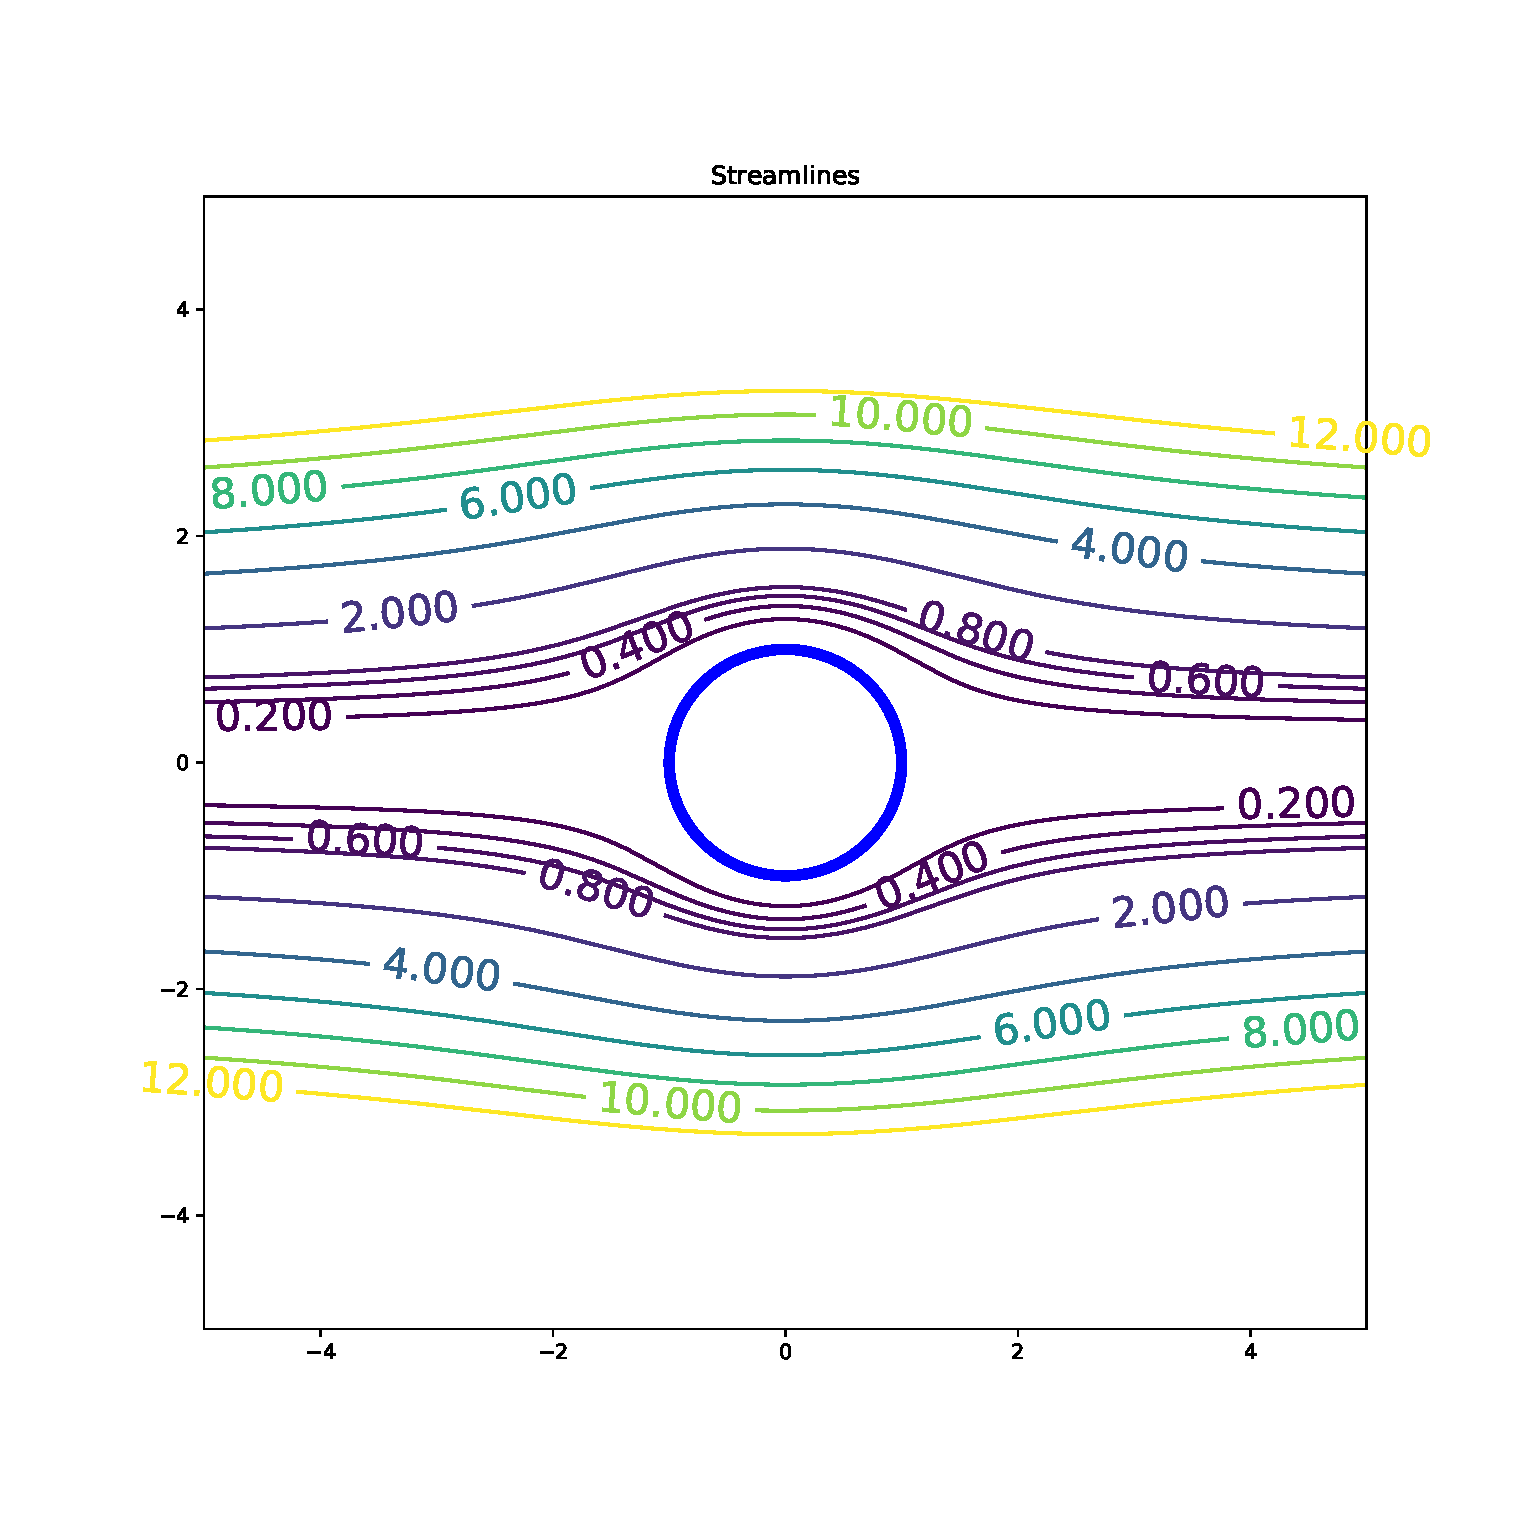
\includegraphics[width=0.8\linewidth]{figures/creeping_flow_past_sphere}
  \caption{\label{fig:creeping_flow_past_sphere}}
\end{figure}


\begin{figure}
  \centering
  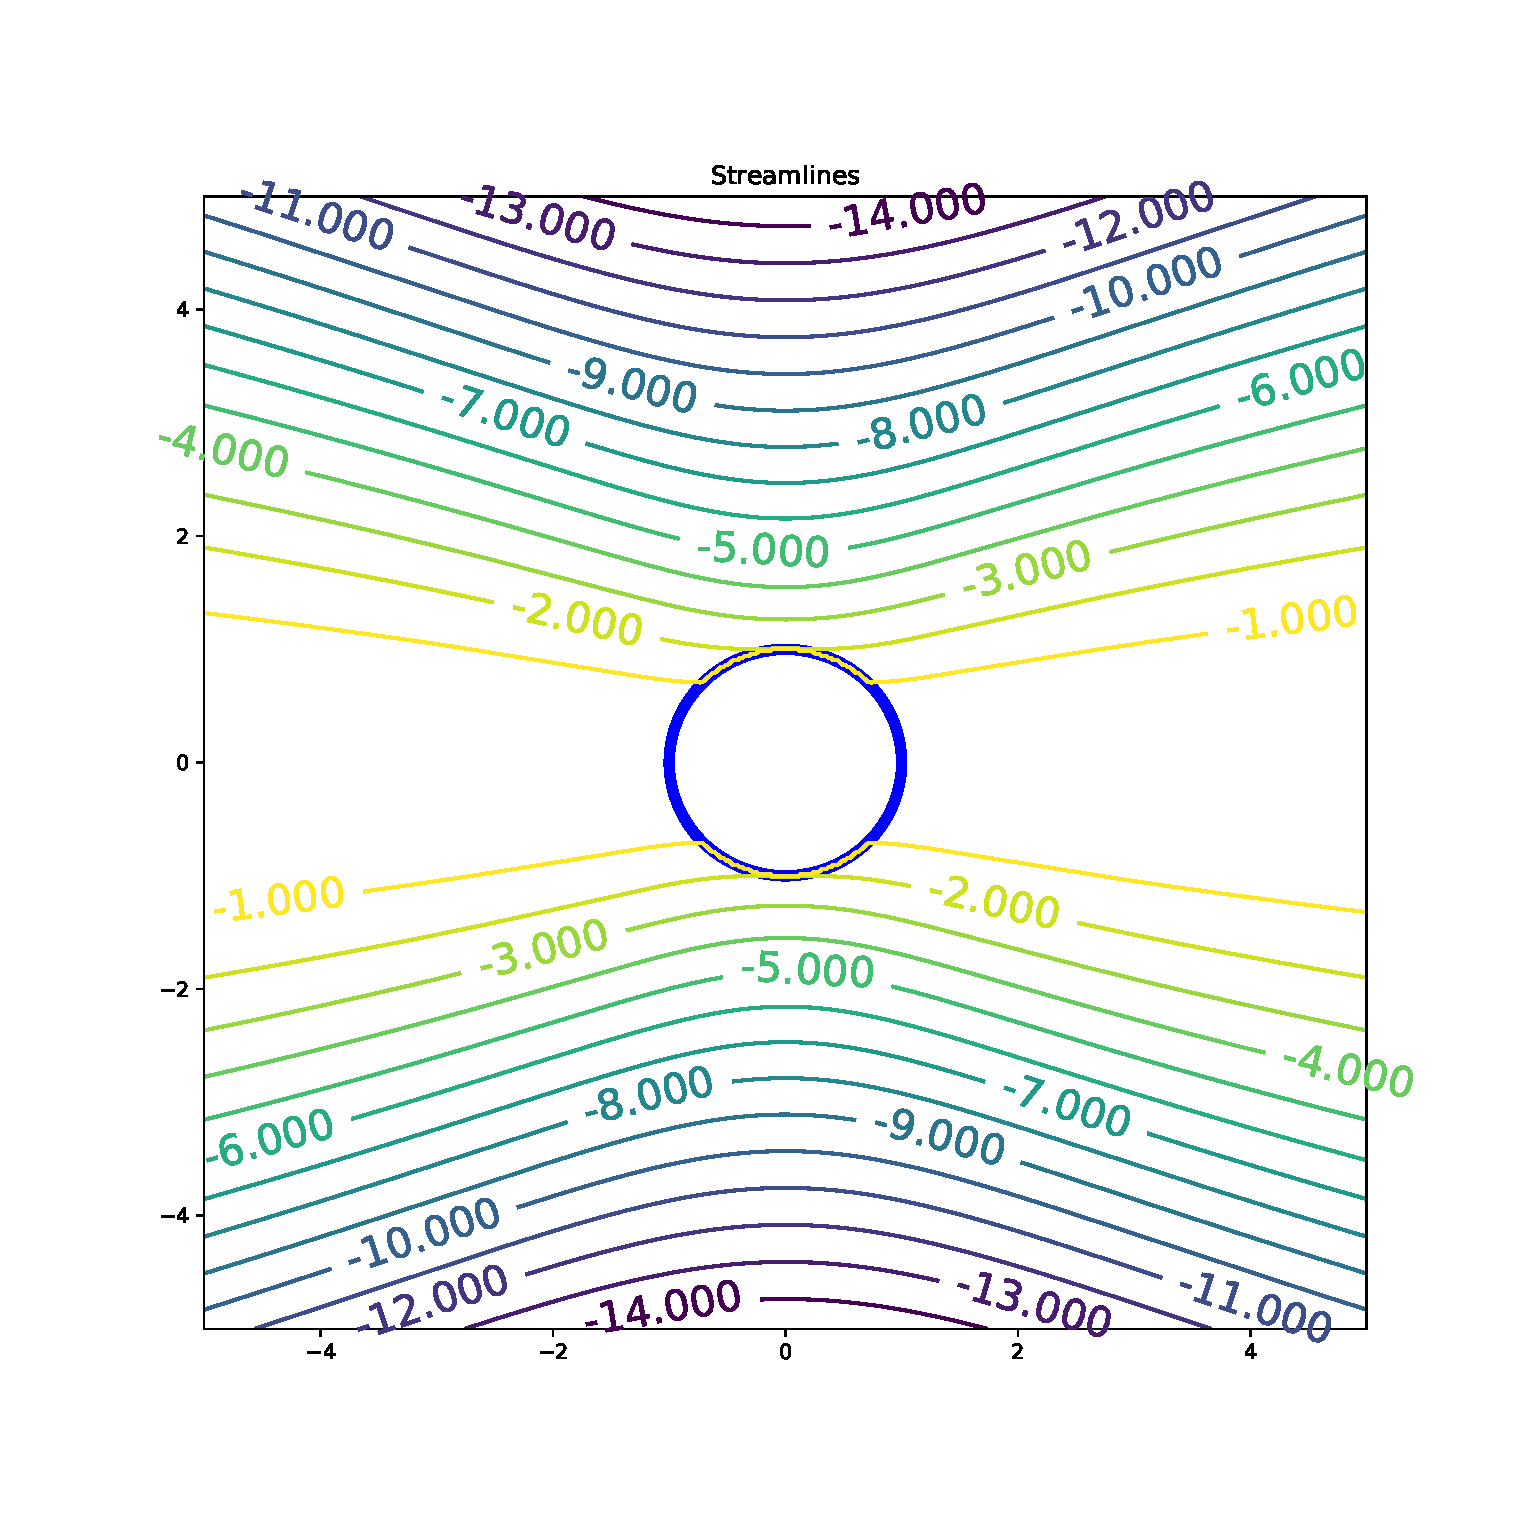
\includegraphics[width=0.8\linewidth]{figures/creeping_flow_past_sphere_moving}
  \caption{\label{fig:creeping_flow_past_sphere_moving}}
\end{figure}



% to be merged onto creeping.tex

If we try $\psi=r^2 \sin^2\theta$ we find
\[
  {\cal L} \psi = \left[ a(a-1) - 2 \right] r^{a-2} \sin^2\theta ,
\]
so the possible exponent values for ${\cal L} \psi = 0$ are $a=2$ and
$a=-1$ (this basically solves the potential flow problem.)

Notice that, once again, the outcome contains a function that is very
similar to the input. This means that, applying twice the differential
operator we will get
\[
  {\cal L}^2 \psi =
  \left[   a  (a-1) - 2 \right]
  \left[ (a-2)(a-3) - 2 \right]
  r^{a-4} \sin^2\theta ,
\]
so  the possible exponent values for ${\cal L}^2 \psi = 0$ are $a=2$ and
$a=-1$, as before, plus $a=4$ and $a=1$.

The solution we try will be a combination of all four posibilities --- but
the $a=4$ we can discard right away because it is too high a divergence. Let
us write
\[
  \psi = u_0 \left[ \frac12 r^2 + \frac{A}{r} + B r \right] \sin^2\theta .
\]
Then our boundary conditions at $r=R$ imply
\begin{align*}
  \left.\frac{\partial \psi}{\partial r}\right|_{r=R} = 0 &\implies
                                                            R-\frac{A}{R^2} + B  =0 \\
  \left.\frac{\partial \psi}{\partial \theta}\right|_{r=R} = 0 &\implies
                                                            \frac12 R^2-\frac{A}{R} + BR  =0 ,
\end{align*}
from which we may obtain $A$ and $B$, and finally write the solution
\[
  \psi = \frac12 u_0 R^2
  \left[\left(  \frac{r}{R} \right)^2
    + \frac12 \frac{R}{r} - \frac32 \frac{r}{R} \right] \sin^2\theta .
\]
The components of the velocity are readily found from
\ref{eq:u_from_psi_spherical},
\begin{equation*}
  \begin{split}
    u_r     &=  u_0  \left[
      1+ \frac12 \left(\frac{R}{r}\right)^3 - \frac32 \frac{R}{r}
    \right] \cos \theta \\
    u_\theta &=
    - u_0  \left[
      1
      - \frac14 \left(\frac{R}{r}\right)^3 - \frac34 \frac{R}{r}
    \right] \sin \theta
  \end{split}
\end{equation*}

The pressure is found from \ref{eq:}, and found to have a simple expression,
\[
  p=p_0 - \frac32 \frac{\mu u_0}{R} \left(\frac{R}{r}\right)^2
  \cos\theta ,
\]
where $p_0$ is the pressure far from the sphere. Notice this pressure
is harmonic, as discussed above. At the sphere surface,
\[
  p(r=R) = p_0 - \frac32 \frac{\mu u_0}{R} \cos\theta,
\]
with a high-pressure zone at the fore of the sphere (the point facing
the upstream direction, $\theta=\pi$), and a lower pressure at the aft
($\theta=0$). This clearly asymmetric pressure distribution results in
a net drag on the sphere
\[
  D_p=  - \int_S  p \cos\theta dA =
  -2\pi R^2 \int_0^\pi d\theta \sin\theta  p(\theta) \cos\theta =
  + 3 \pi \mu u_0 R \int_0^\pi d\theta \sin\theta  \cos^2\theta .
\]
The minus sign comes from the fact that we want the pressure upon the
sphere, which by reaction is opposite the pressure upon the fluid.
The last integral is immediate: the primitive is $-(1/3)\cos^3\theta$,
so the definite integral provides a $2/3$ factor. Finally,
\[
  D_p=  2 \pi \mu u_0 R .
\]
This agrees with our guess of \ref{eq:drag_sphere_guess}.

However, this drag force is due to pressure only. There will be an
additiona shear drag, which may be calculated from the shear stress.
The relevant component of the tensor is (see \cite{white1991viscous},
Eq. B17, p. 584):
\[
  \tau_{r\theta} = \mu \left(
    \frac1r
    \frac{\partial u_r}{\partial \theta} +
    r \frac{\partial }{\partial r} \left( \frac{u_\theta}{r}\right) 
  \right) .
\]

This can be computed to obtain
\[
  \tau_{r\theta} = 
  - \frac32 \frac{\mu u_0}{r} \left(\frac{R}{r}\right)^3 \sin\theta ,
\]
hence at the sphere surface,
\[
  \tau_{r\theta} (r=R) =  - \frac32 \frac{\mu u_0}{R}  \sin\theta .
\]
This looks very similar to the pressure, with a $\sin$ instead of a
$\cos$, which means the stress is maximal at the equator, which seems
reasonable. However, the contribution to the drag force is higher ---
twice higher, to be precise. Indeed,
\[
  D_\tau =  - \int_S  \tau_{r\theta} \sin\theta dA ,
\]
with a minus sign for the same reason as the pressure, and a $\sin$
because this is a shear stress, resulting in a force that is
tangential to the surface of the sphere.  Then
\[
  D_\tau =
  - 2\pi R^2 \int_0^\pi d\theta   \tau_{r\theta} \sin^2\theta  =
  3 \pi \mu u_0 R  \int_0^\pi d\theta \sin^3\theta .
\]
The primitive of $\sin^3\theta$ is, through
$\cos^2\theta=1-\sin^2\theta$, equal to
$(1/3) \cos^3\theta - \cos\theta$. The definite integral is then $4/3$, and
\[
  D_\tau = 4 \pi \mu u_0 R .
\]

The final drag force is the celebrated Stokes drag law: \index{Stokes drag law}
\[
  D_\tau = 6 \pi \mu u_0 R ,
\]
where $1/3$ of the drag is due to pressure and $2/3$ to shear stress.

Despite the shear having a contribution that is twice that two
pressure, notice that by writing 
\begin{align*}
  - p(r=R) + p_0 &= \bar{p} \cos\theta,  
  -\tau_{r\theta} (r=R) &= \bar{p} \sin\theta,  
\end{align*}
where $\bar{p} := - (3/2) \frac{\mu u_0}{R}$, it is apparent that the
normal force, due to pressure, and the tangential one, due to shear
stress, result from a decomposition of a force upon the sphere surface:
\[
  \bff := \frac32 \frac{\mu u_0}{R} \bhe_z .
\]
It is remarkable that this force is equal for every point on the
sphere.




FOR POTENTIAL.TEX:




In axisymmetric flow,
\[
  \divu =
  {1 \over r^2}{\partial \left( r^2 u_r \right) \over  \partial r} +
  {1 \over r\sin\theta}{\partial \over \partial  \theta} \left( u_\theta\sin\theta \right) ,
\]
but an equivalent expression is
\[
  \divu =
  {\partial \left( r^2 u_r \sin\theta \right) \over  \partial r} +
  {\partial \left( r u_\theta\sin\theta \right)  \over \partial  \theta}
\]

so continuity is trivially satisfied with the choice
\ref{eq:u_from_psi_spherical}.


From the curl in spherical coordinates,
\begin{align}
  u_r     &= \frac {1}{r\sin \theta }
            \frac{ \left( \partial A  \sin \theta \right) }{\partial \theta }  \\
  u_\theta &= -\frac1{r} \frac{\partial (rA) }{\partial r} 
\end{align}
and we find
\begin{equation}
%  \label{eq:u_from_psi_spherical}
  \begin{split}
    u_r     &=  \frac1{r^2 \sin\theta} \frac{\partial \psi}{\partial \theta} \\
    u_\theta &= -\frac1{r   \sin\theta} \frac{\partial \psi}{\partial r}
  \end{split}
\end{equation}



Notice $A=\psi / \rho $ also in spherical coordinates !
